\RequirePackage{fix-cm}
\documentclass[conf]{new-aiaa}

\usepackage[utf8]{inputenc}
\usepackage{hyperref}
\usepackage{graphicx}
\usepackage{siunitx}
\sisetup{group-separator = {,}}
\usepackage{booktabs}
\usepackage{enumitem}
\usepackage{float}
\usepackage{amsmath}
\usepackage[version=4]{mhchem}
\usepackage{longtable,tabularx}
\usepackage{placeins}
\usepackage{multirow}
\usepackage{booktabs}
\usepackage{latexsym}
\usepackage{subcaption}
\usepackage{latexsym}
\usepackage[sort&compress,numbers]{natbib} % For bibtex \citet, \citep
\usepackage{hypernat} % To get natbib to play nicely with hyperref
\usepackage{doi} % For getting hyperlinked DOI in the references


\hypersetup{
    pdfauthor={Peter Atma}, % insert author here
	pdftitle={Aviation 2022 Abstract}, % insert title here
	pdfsubject={Propulsion Analysis and Optimization of a High Bypass Turbofan Engine}, % insert keywords here
}

\graphicspath{{../figures/}}

\title{Multi-point Low-Emission Propulsion Analysis and Optimization of a High Bypass Turbofan Engine} % change

\author{Peter Atma\footnote{MSE Student, Department of Aerospace Engineering, AIAA Student Member}}
\author{Andrew H.R. Lamkin\footnote{Ph.D.~Candidate, Department of Aerospace Engineering, AIAA Student Member}}
\author{Joaquim R.~R.~A.~Martins\footnote{Professor, Department of Aerospace Engineering, AIAA Fellow}}
\affil{University of Michigan, Ann Arbor, MI, 48109}

% ==================================================
%	Abstract
% ==================================================

% ==================================================
\begin{document}

\maketitle

\begin{abstract}
	Advances in commercial propulsion technology has lead to the development of larger and more advanced high-bypass turbofan engines with larger bypass ratios, pressure ratios, and internal temperatures.
	With the impending climate crisis, aircraft and engine manufacturers have been pushing for greener fuels and more efficient engines to lower greenhouse and NOx emissions.
	This has revitalized research into using liquid hydrogen as a fuel for aircraft turbine engines in addition to using known thrust augmentation techniques to reduce NOx emissions and improve fuel efficiency.
	The high-bypass turbofan study investigates the industry-proposed benefits of using a closed-loop water injection and water vapor recovery system with two types of fuels.
	We will perform a single point analysis to explore the design space and a multi-point gradient-based optimization to determine and validate the efficiency and emission improvements associated with the proposed engine model.
	Finally, we will present the results from the design space analysis and multi-point optimization from this model. These developments will accelerate and validate current research into the next generation of fuel-efficient, low emission high-bypass turbofan engines.
\end{abstract}

\section{Introduction}
% Message 1: Motivation to incorporate low-emission fuels and techniques
In the commercial aviation industry today, the global effects of climate change and high gas prices have motivated the development of more efficient and cleaner propulsion systems.
Most development so far has been targeted at making existing engine architectures more efficient with the fuels and technologies we currently have to reduce fuel consumption and thus release fewer carbon and NOx emissions.
By continuing this trend of development, high-bypass turbofan engines can be improved by lowering the pressure ratio of the fan to enable a higher bypass ratio of the engine.
Furthermore, higher overall pressure ratios and more advanced metals with higher melting temperatures can allow larger burner temperatures both of which improve thermal efficiency.

Additionally, greener fuels can be used that have fewer products that are harmful to the environment and human health.
Liquid hydrogen has been proposed as a possible replacement fuel for hydrocarbon fuel such as Jet-A due to the fact that hydrogen has zero carbon emissions and the combustion products mainly consist of water vapor.
A consequence of using hydrogen as a fuel and designing higher pressure ratios is that hydrogen burns at higher temperatures than hydrocarbon fuels and higher pressure ratios result in higher combustion pressures.
High combustion temperatures and pressures tend to increase NOx formation and emissions in aircraft engines.

% Message 2: Background and references to support using H2 and water injection in HBTF engines
Therefore, a potential solution to these downsides is to inject finely atomized water droplets into the core air stream of a high-bypass turbofan engine.
While water injection is generally an old technology, studies conducted by NASA, Boeing, and Rolls-Royce suggest that this technique can be used to reduce the NOx emissions in high-bypass turbofan engines by as much as 47\%.
Additional benefits include improvements in fuel efficiency and thrust, lower burner temperatures to improve the lifetime of high-temperature components, and engine noise reduction \cite{nasa_inject}.
While water injection may provide all of these benefits, water would still have to be stored on the aircraft and increase the weight of the aircraft.
Therefore, a method currently being investigated in industry is to use a closed-loop system that uses water vapor recovery from the exhaust to provide the water for injection.
This would eliminate the need for a water reservoir that would decrease the overall aircraft performance.

These potential efficiency and emission improvements of aircraft engines can be cheaply and efficiently evaluated by using one-dimensional cycle analysis.
One-dimensional cycle analysis uses a first-principles approach with simplifying assumptions to provide a low-fidelity model for engine analysis.
This can be used to understand the general trends and design constraints of a engine cycle and evaluate potential improvements in design. Current tools that exist for engine cycle analysis include Numerical Propulsion System Simulation (NPSS) and pyCycle.
NPSS utilizes a modular object-oriented framework in which individual engine components are connected and thermodynamic properties are evaluated using Chemical Equilibrium with Applications (CEA) to determine performance metrics of a given design.
pyCycle improves on this modular architecture by introducing efficient analytic gradients to allow gradient-based multidisciplinary optimization \cite{Hendricks2019}.

% Message 3: Introduce the extension of the HBTF and propose novel contributions
In this work, we will analyze the potential propulsion benefits of closed-loop water vapor recovery with water injection in a high-bypass turbofan engine by optimizing the thrust-specific fuel consumption (TSFC) with a NOx emission constraint.
This will be accomplished by developing new pyCycle components for water injection and vapor recovery and will use empirical NOx formation correlations to evaluate NOx emissions.
Furthermore, two fuel types will be evaluated, Jet-A and liquid hydrogen to determine the maximum improvement of engine performance over current technologies.

In Section \ref{sec:epModel} we introduce the turbofan model and explain how we will introduce the water injection and water recovery components within the model.
Section \ref{sec:imp} explains how the multidisciplinary optimization will be implemented to take into account the different operating conditions of the engine model and the associated NOx emissions.

\section{Emission-Propulsion Model Description}
\label{sec:epModel}
% Engine Architecture: Describe the flow path of the engine and establish the mechanical coupling.
We will use a next-generation high-bypass turbofan engine configuration for this work.
Specifically, the NASA advanced technology high bypass geared turbofan engine cycle, referred to as the "N+3" engine, was selected for this research \cite[]{Hendricks2019}. The N+3 reference cycle represents a notional high bypass ratio geared turbofan that could be available in the 2030–2040 time frame.
This engine was selected since it has already been modeled in pyCycle as a robust example cycle and includes the advanced engine cycle improvements that were mentioned before such as a large bypass ratio, high pressure ratio, and high combustion temperature.
This model consists of an inlet that directs ambient air through a fan, followed by a duct that splits the flow into a core flow and a bypass flow, and ends in a bypass nozzle and core nozzle. The fan and low pressure compressor (LPC) are connected to the low pressure turbine (LPT) by the low pressure shaft.
Similarly, the high pressure compressor (HPC) is connected to the high pressure turbine (HPT) by the high pressure shaft. Along the axial flow path, a the one-dimensional thermodynamic connections are solved using CEA to ensure first the principle governing equations are satisfied.
We then introduce a water injection component directly before the HPC.
This will inject pure water vapor into the core stream to reduce the flame combustion temperature.
The water vapor recovery component is then introduced directly before the core nozzle to recover water vapor from the core stream.
While in practice this component would require a technical analysis of a condenser in the core stream, this work is only looking at the potential benefit of extracting water vapor and not the recovery method specifically.
With these components integrated into the N+3 engine, the coupled water inject and water recovery presents a implicit relationship which would need to be iterative solver to match the flow rate entering the engine and exiting the engine.
The flow and mechanical connections within the engine model with the water injector and water extractor are visualized in Figure \ref{fig:hbtf_cycle}.

\begin{figure}[H]
	\centering
	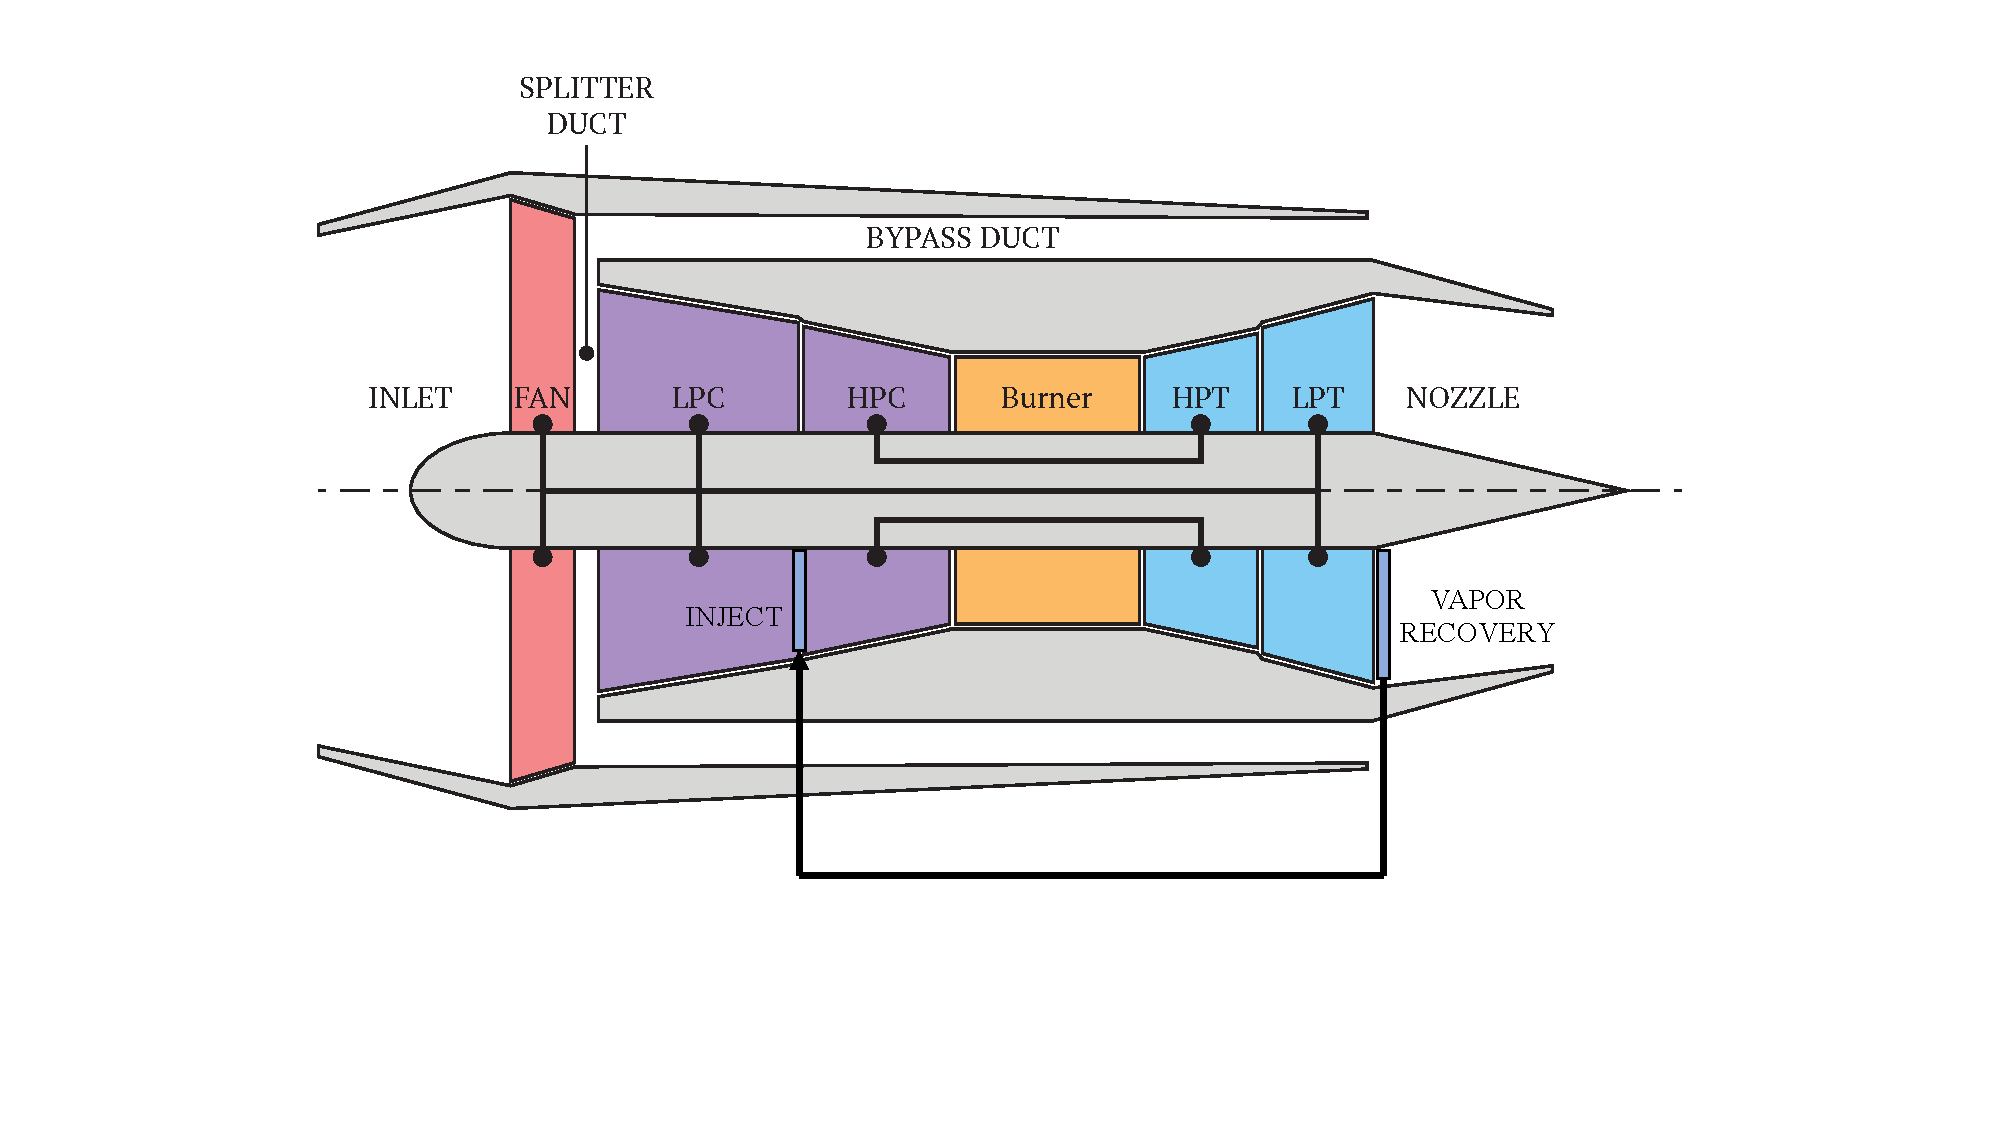
\includegraphics[width=0.8\textwidth]{turbofan_wvr.pdf}
	\caption{Configuration of the high-bypass turbofan model with vapor recovery and injection.}
	\label{fig:hbtf_cycle}
\end{figure}

% Preliminary Results
This model has been tested using Jet-A and liquid hydrogen fuels to determine the improvements in efficiency with injecting water into the core stream.
Preliminary results are shown in Figure \ref{fig:results} and show the relative improvement in thrust specfic energy consumption with water injection for the same engine design with each type of fuel.
We can already see great improvements in the cruise engine efficiency which may be able to be further improved with a full engine optimization.

\begin{figure}[H]
	\centering
	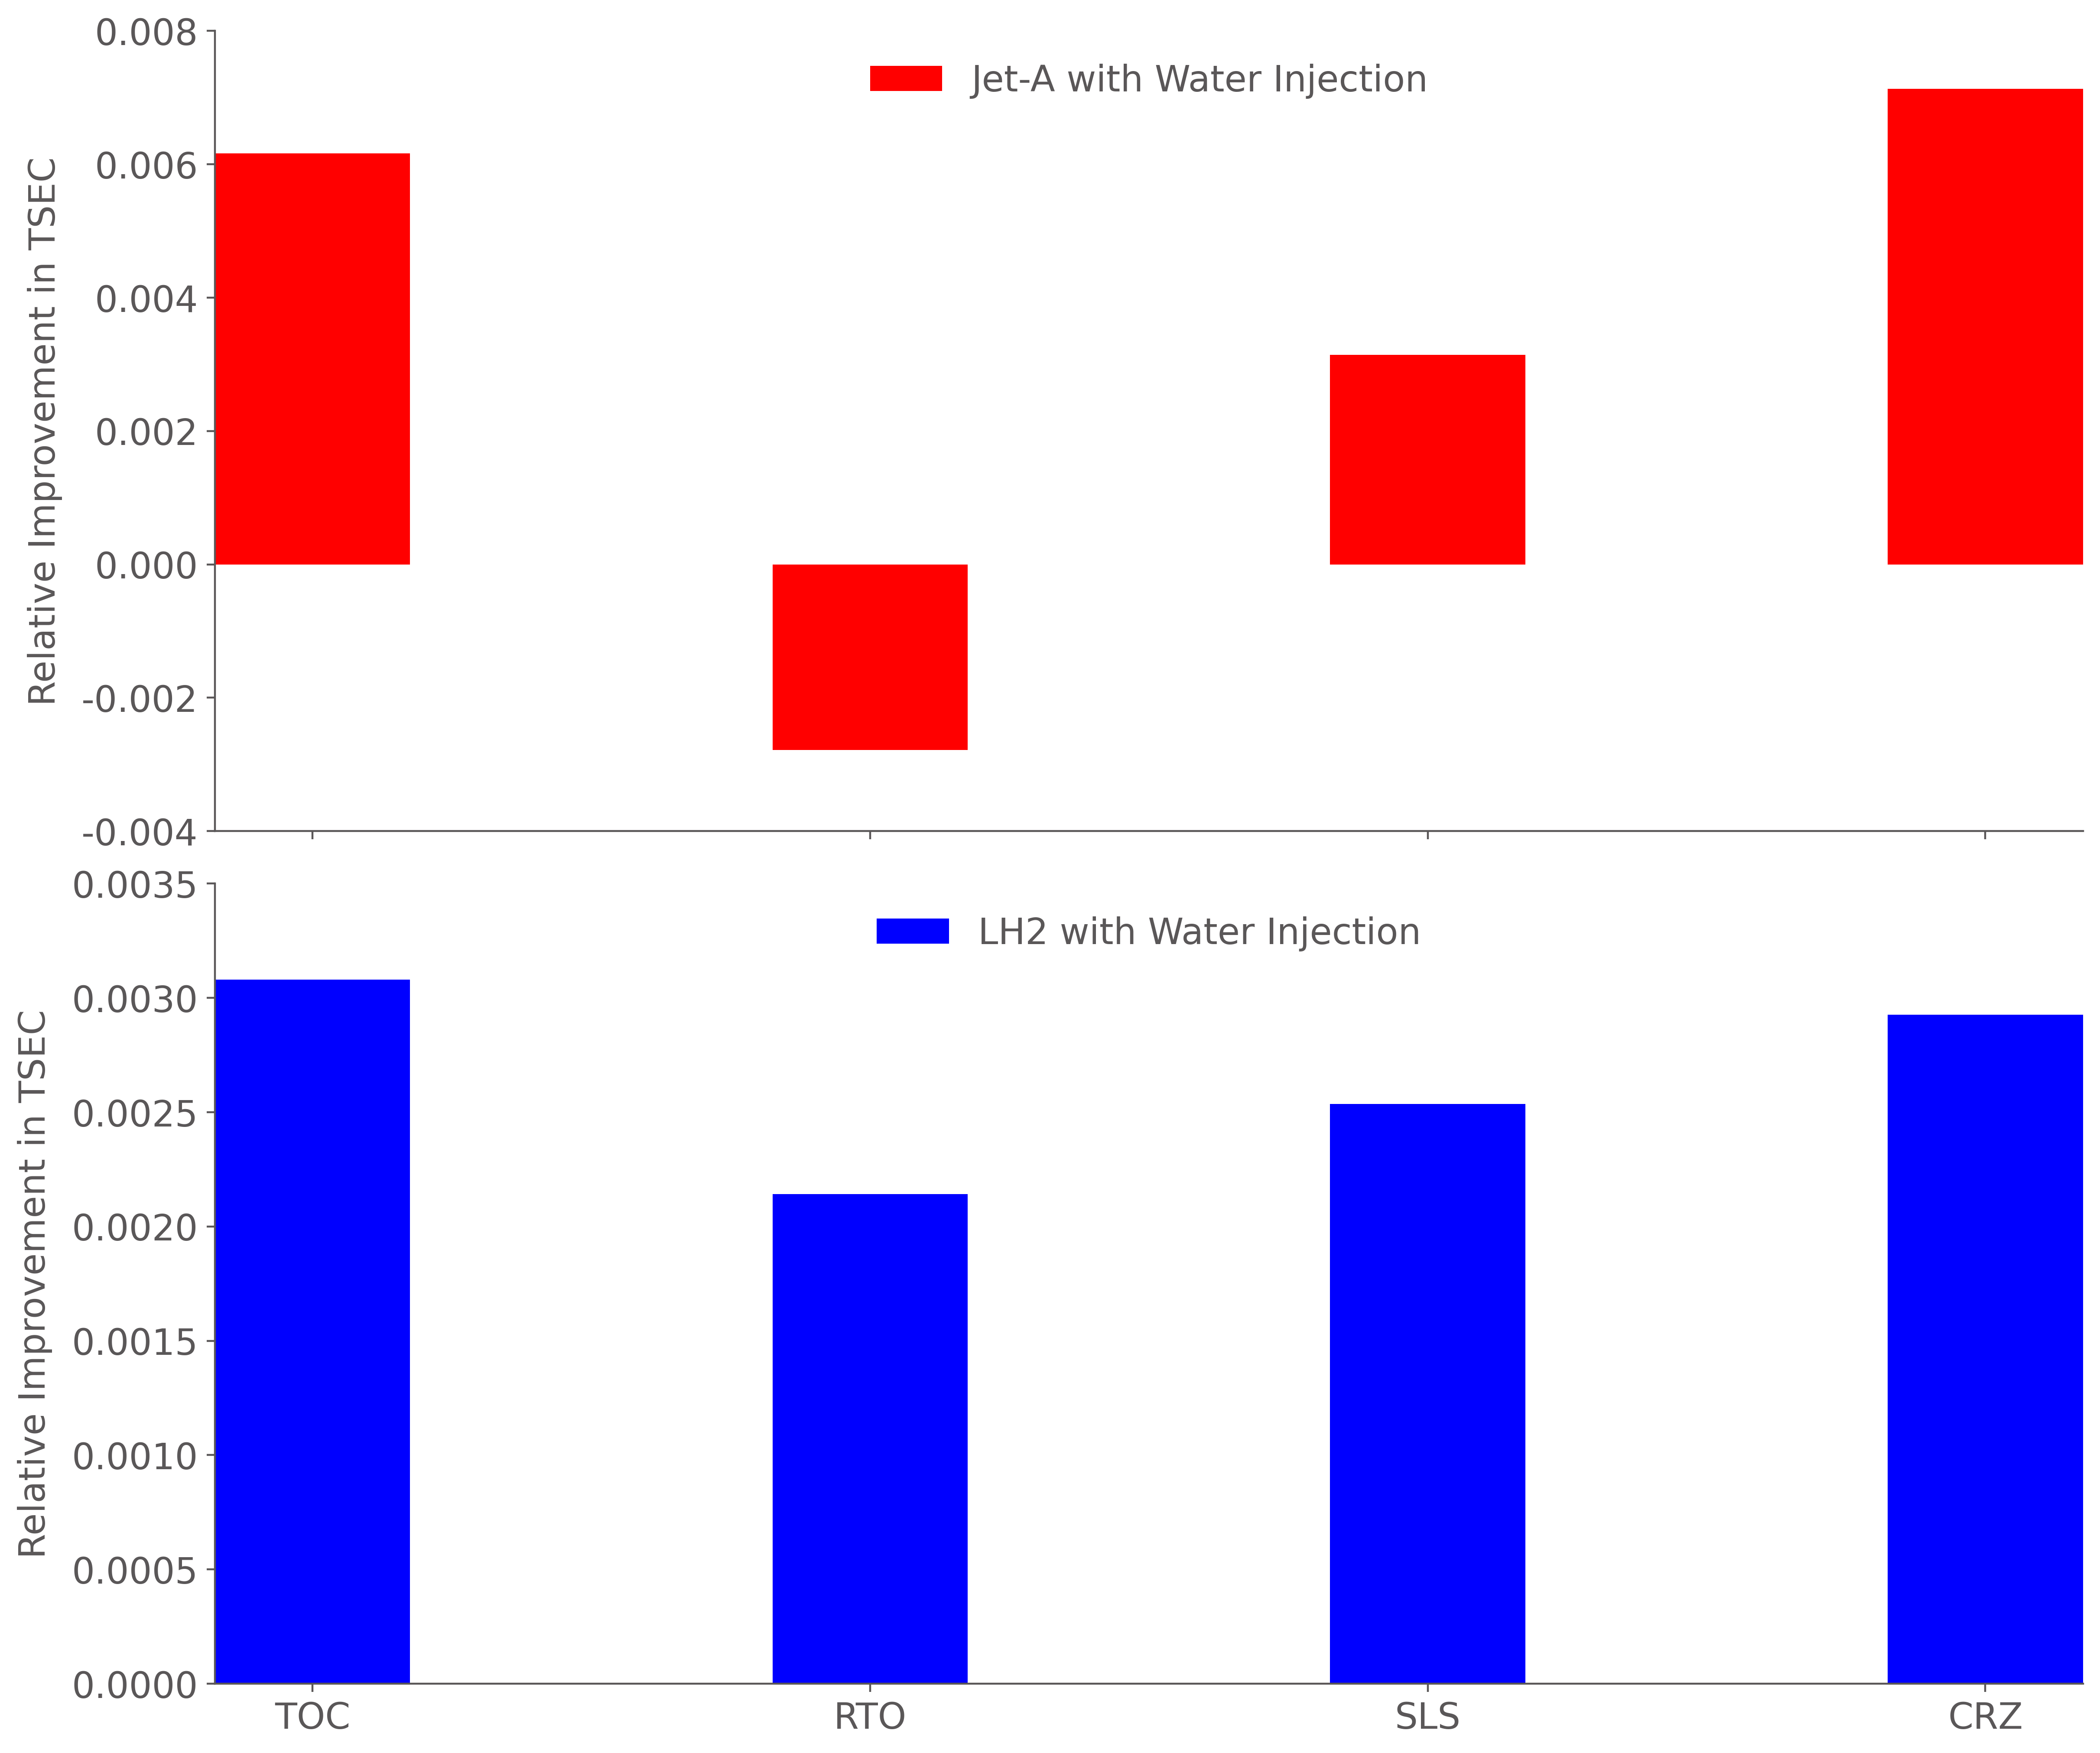
\includegraphics[width=0.8\textwidth]{JetA-H2_bar_chart_diff.png}
	\caption{Relative improvement in TSEC from water injection.}
	\label{fig:results}
\end{figure}

\section{Implementation}
\label{sec:imp}
% Fully coupled model
The propulsion model is constructed in pyCycle which is built on top of OpenMDAO to allow a modular design of the engine components and allows the coupling of other engineering disciplines for analysis \cite{Gray2019a}.
For the Jet-A fuel, the NOx correlation will use the P3-T3 method which is commonly a used technique in industry to determine NOx formation in aircraft engines while considering humidity \cite[]{Dubois2006}.
This method uses the pressure and temperature of the flow before the combustor to determine NOx formation from a reference design condition of the engine.
Since not many NOx correlations exist for the NOx formation for the liquid hydrogen fuel, we will use a surrogate model using data computed using Cantera to approximately model the NOx emissions.

% Briefly discuss the optimization problem
We will perform gradient-based emission-propulsion design optimization of the engine model with a multipoint architecture that considers the common flight conditions experienced by commercial aircraft. And XDSM diagram of the optimization problem is shown in Figure \ref{fig:opt_prob}.

\begin{figure}[H]
	\centering
	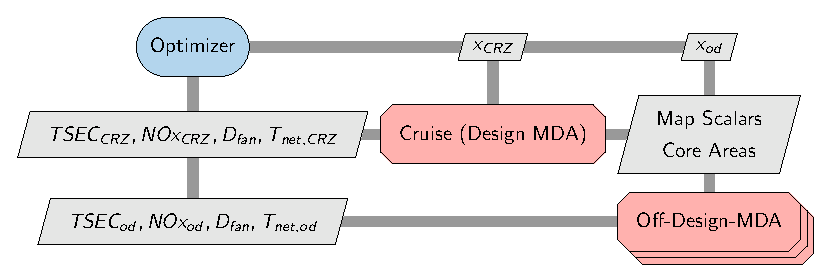
\includegraphics[width=0.8\textwidth]{N3_inject.pdf}
	\caption{XDSM diagram of the multi-point optimization problem with constraints.}
	\label{fig:opt_prob}
\end{figure}

The objective is to minimize the thrust specific energy consumption at a cruise condition subject to NOx formation, thrust, engine diameter.
Following this study, we will conduct a multi-objective optimization problem considering thrust specific fuel consumption and NOx formation.
This will define a pareto front of different thrust specific fuel consumption and NOx formation designs to show trade-offs in the design space.

\section{Conclusion}
% Message 1: Re-state the problem
In this work, we will model, analyze, and optimize a high-bypass turbofan propulsion cycle using a novel closed-loop water vapor recovery to improve cycle efficiency and NOx emissions. We
% Message 2: Summarize the HBTF model
The high-bypass turbofan engine will be composed of separate sub-components modeled in pyCycle with two newly developed water injection and water vapor recovery components to accurately compute the thermodynamic response of the engine.
Two fuels, Jet-A and liquid hydrogen, will be compared with and without the closed-loop water vapor recovery system to determine the benefits of the implementation.
NOx formation will be modeled using common industry methods and a novel reactor model in Cantera for hydrogen combustion NOx formation.
% Message 3: Expected results
The results will include a full propulsion-emission analysis of the novel systems with multipoint design optimizations of the entire flight envelope.
This work will build off of current industry research into NOx emission reduction methods and provide a first principles analysis of the potential benefits of closed-loop water vapor recover and injection for commercial aviation applications.

\bibliography{mdolab,references}

\end{document}
